\documentclass[11pt,a4paper,dvipdfmx]{jsarticle}
%
\usepackage{amsmath,amssymb}
\usepackage{bm}
\usepackage{graphicx}
\usepackage{ascmac}
\usepackage{csvsimple}
\usepackage{pdfpages}
\usepackage{hyperref}
%
\setlength{\textwidth}{\fullwidth}
\setlength{\textheight}{40\baselineskip}
\addtolength{\textheight}{\topskip}
\setlength{\voffset}{-0.2in}
\setlength{\topmargin}{0pt}
\setlength{\headheight}{0pt}
\setlength{\headsep}{0pt}
%
\hypersetup{% hyperrefオプションリスト
setpagesize=false,
 bookmarksnumbered=true,%
 bookmarksopen=true,%
 colorlinks=true,%
 linkcolor=blue,
 citecolor=blue,
}
%
\newcommand{\divergence}{\mathrm{div}\,}  %ダイバージェンス
\newcommand{\grad}{\mathrm{grad}\,}  %グラディエント
\newcommand{\rot}{\mathrm{rot}\,}  %ローテーション
%
\title{計算数学2レポート}
\author{西原寛人 1823123s}
\date{2021年7月21日更新(2021年7月17日作成)}
\begin{document}
\maketitle
%
%
%メモ:csvをtabular(TeXで使える表敬式)に変換するにはhttps://rra.yahansugi.com/scriptapplet/csv2tabular/index.html
%が便利
%
%
%
\section{用いるデータ}
 プロ棋士の戦型別の勝率データを用いて、棋士の強さや戦型ごとの強さを分析した。
データは将棋棋士成績DB(http://kenyu1234.php.xdomain.jp/menu.php)からとった。
\\
\begin{tabular}{c||c|c|c|c|c|c|c|c|c} 
    & yag & yoko & kk & aig & airiki & vs2 & vs3 & vs4 & vs5 \\ \hline
    habu & 0.7161 & 0.6824 & 0.625 & 0.6913 & 0.5833 & 0.7037 & 0.8136 & 0.7771 & 0.7563 \\
    fuziis & 0.9123 & 0.6111 & 0.8209 & 0.7714 & 0.8889 & 0.8929 & 0.9231 & 0.84 & 0.8929 \\
    watanabe & 0.6723 & 0.6395 & 0.6987 & 0.662 & 0.6667 & 0.7 & 0.6071 & 0.6515 & 0.6 \\
    satouy & 0.6272 & 0.6053 & 0.5054 & 0.5732 & 0.3846 & 0.7333 & 0.717 & 0.6644 & 0.6235 \\
    sugai & 0.6786 & 0.7826 & 0.6154 & 0.25 & 0.6364 & 0.7 & 0.75 & 0.5 & 0.6667 \\
    kubo &  &  &  &  &  &  &  & 0.7368 &  \\
    suzuki & 0.4286 &  &  &  &  &  &  &  &  \\
    fuziit & 0.537 &  &  &  & 0.5556 &  & 0.8333 & 0.5556 &  \\
    saitou & 0.6914 & 0.7059 & 0.5625 & 0.5714 & 0.4 & 0.5385 & 0.7273 & 0.7368 & 0.7895 \\
    toyoshima & 0.6631 & 0.6953 & 0.6769 & 0.625 & 0.7778 & 0.7692 & 0.55 & 0.6958 & 0.6341 \\
    hirose & 0.5765 & 0.6316 & 0.5439 & 0.4545 & 0.7 & 0.7619 & 0.6875 & 0.6538 & 0.6667 \\
    itotani & 0.5714 & 0.62 & 0.5851 & 0.5292 & 0.7826 & 0.7857 & 0.6111 & 0.5833 & 0.7714 \\
    satoua & 0.6456 & 0.6967 & 0.5513 & 0.5833 & 0.4375 & 0.8065 & 0.6923 & 0.8065 & 0.6286 \\
    nagase & 0.6923 & 0.7538 & 0.6786 & 0.7333 & 0.6364 & 0.75 & 0.6875 & 0.84 & 0.8077 \\
    yamazaki & 0.6286 & 0.618 & 0.5636 & 0.5904 & 0.7097 & 0.7619 & 0.6316 & 0.6792 & 0.7105 \\
    inaba & 0.6491 & 0.5319 & 0.619 & 0.5439 & 0.3636 & 0.5909 & 0.5714 & 0.6786 & 0.7292 \\
    miura & 0.5668 & 0.4892 & 0.4741 & 0.675 & 0.6667 & 0.3636 & 0.5814 & 0.5325 & 0.5938 \\
    kimura & 0.538 & 0.5789 & 0.5854 & 0.5979 &  & 0.4571 & 0.697 & 0.6829 & 0.6774 \\
    gouda & 0.6058 & 0.5135 & 0.4991 & 0.6667 &  & 0.6563 & 0.7436 & 0.6691 & 0.5676 \\
    kondou & 0.6923 & 0.5883 & 0.6346 & 0.6341 & 0.6667 & 1 & 0.5 & 0.7 & 0.5714 \\
    senda & 0.6588 & 0.6471 & 0.6753 & 0.75 & 0.8 & 0.6667 & 0.8 & 0.68 & 0.72 \\
    yashiki & 0.5572 & 0.5102 & 0.4359 & 0.5748 &  & 0.5385 & 0.7381 & 0.6286 & 0.6078 \\
    matsuo & 0.5043 & 0.5371 & 0.5361 & 0.5612 & 0.3636 & 0.4583 & 0.65 & 0.6585 & 0.5152 \\
    akutsu & 0.5172 & 0.5426 & 0.44 & 0.4727 & 0.6667 & 0.8571 & 0.6111 & 0.6042 & 0.5952 \\
    sasaki & 0.5775 & 0.75 & 0.5385 & 0.7083 & 0.7778 & 0.8 & 0.5833 & 0.6522 & 0.6957 \\
    yokoyama & 0.65 & 0.6508 & 0.4286 & 0.6129 & 0.6364 & 0.7619 & 0.5385 & 0.7097 & 0.5417 \\
    
    
\end{tabular}

\begin{tabular}{c||c|c|c|c|c|}
    & 2 & 3 & 4 & 5 & aifuri \\ \hline
    habu & 0.6 & 0.4286 & 0.6757 & 0.6222 &  \\
    fuziis &  &  &  &  &  \\
    watanabe &  &  & 0.3571 & 0.5 &  \\
    satouy & 0.5259 & 0.5455 & 0.64 & 0.5106 & 0.4865 \\
    sugai & 0.7333 & 0.717 & 0.4667 & 0.6554 & 0.697 \\
    kubo & 0.5435 & 0.5706 & 0.585 & 0.5507 & 0.6165 \\
    suzuki & 0.5 & 0.5288 & 0.4613 & 0.6229 & 0.5275 \\
    fuziit & 0.6429 & 0.6447 & 0.5679 & 0.4275 & 0.5816 \\
    saitou &  &  &  &  & 0.6667 \\
    toyoshima &  & 0.5455 &  & 0.8077 & 0.4667 \\
    hirose &  & 0.6875 & 0.6638 & 0.678 & 0.7273 \\
    itotani & 0.6111 &  &  & 0.3077 &  \\
    satoua &  & 0.4163 &  & 0.5556 & 0.875 \\
    nagase &  & 0.7097 & 0.7143 & 0.5952 & 0.7368 \\
    yamazaki & 0.5556 & 0.4 & 0.3333 & 0.6667 & 0.4762 \\
    inaba &  &  &  & 0.7273 & 0.8571 \\
    miura & 0.5882 & 0.381 & 0.5946 &  &  \\
    kimura & 0.4571 &  &  &  &  \\
    gouda &  &  &  &  &  \\
    kondou &  &  &  &  &  \\
    senda &  &  &  &  & 0.8 \\
    yashiki & 0.4667 &  & 0.6 & 0.5625 &  \\
    matsuo &  &  & 0.5556 & 0.5385 & 0.44 \\
    akutsu & 0.65 & 0.4286 & 0.5897 & 0.6 & 0.7143 \\
    sasaki &  & 0.5714 &  &  & 0.875 \\
    yokoyama &  & 0.52 & 0.5714 & 0.5714 & 0.6667 \\
    
\end{tabular}
\\
\\
\\
 勝数でデータをとると対戦回数の多いベテラン棋士が有利になるので
勝率でデータをとった。
\\
 指した回数が全体の1%未満の戦型は回数が少なすぎて勝率が1や0になるケースがあり、
それを例えば100戦100勝や100戦0勝と同じ強さだと扱うのは良くないので、
指したことがないとみなして空欄とした。
また、採用した場合も対戦相手やそのときの流行との兼ね合いで奇襲の意味合いが強いと思われる。
今回の解析では棋士の強さや戦型自体の強さを分析したいので、不意打ちのような使い方をした対局は省きたい。
普段指さない戦型は普通に指すと強くないと思われるので、biplotで解析するときは勝率を低く仮定し、
零割若しくは三割として分析した。
\\
 将棋の戦型は主に相居飛車、対抗系、相振り飛車の3つに分類される(下図参照)。
\\
\\
\\
\begin{figure}[h]
    \begin{tabular}{cc}
        \begin{minipage}[t]{0.47\hsize}
            \centering
            \includegraphics[width=0.8\textwidth]{graph/shoki.png}
            \caption{初期配置}
        \end{minipage}
        \begin{minipage}[t]{0.47\hsize}
            \centering
            \includegraphics[width=0.8\textwidth]{graph/kk.png}
            \caption{相居飛車(角換わり)}
        \end{minipage}
    \end{tabular}
\end{figure}
\\
\begin{figure}[h]
    \begin{tabular}{cc}
        \begin{minipage}[t]{0.47\hsize}
            \centering
            \includegraphics[width=0.8\textwidth]{graph/taikou.png}
            \caption{対抗系}
        \end{minipage}
        \begin{minipage}[t]{0.47\hsize}
            \centering
            \includegraphics[width=0.8\textwidth]{graph/aifuri.png}
            \caption{相振り飛車}
        \end{minipage}
    \end{tabular}
\end{figure}
\\
 初めの列から飛車を動かさない戦法が居飛車、動かす戦法が振り飛車である(図はすべてShogipic(https://shogipic.jp/)で作成)。
\\
 データのyag、yoko、kk、aig、airikiはそれぞれ矢倉、横歩取り、角換わり、相掛かり、相居飛車力戦の相居飛車の戦型を、
vs2、vs3、vs4、vs5は居飛車で相手がそれぞれ向かい飛車、三間飛車、四間飛車、中飛車の対抗系を、
2、3、4、5はそれぞれ向かい飛車、三間飛車、四間飛車、中飛車で相手が居飛車の対抗系を、
aifuriは相振り飛車を表している。
\\
 今のトップ棋士では居飛車が多用されているので、相居飛車の分類は細かく、相振り飛車の分類は荒くなっている。
\\
 箱ひげ図は以下のようになる。
\begin{figure}[h]
    \centering
    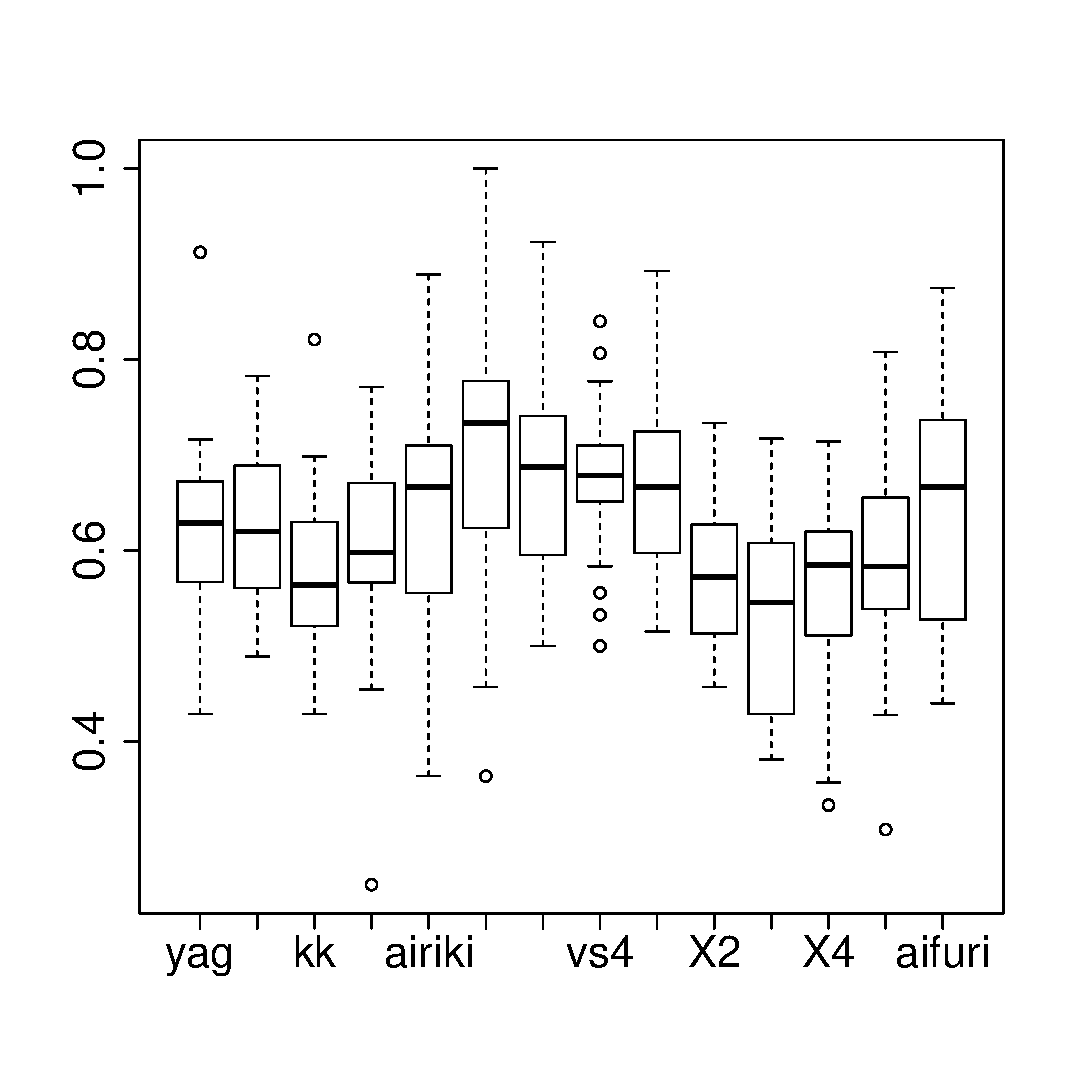
\includegraphics[width=0.45\textwidth]{graph/boxplot-raw.eps}
\end{figure}
\\
\\
 はずれ値は矢倉(yag)、角換わり(kk)で上に抜けて出ているが、これは両方共藤井聡太二冠なので、彼が頭一つ抜けて強いことがわかる。
また対四間(vs4)でも藤井二冠と永瀬王座、佐藤天彦九段が勝率が高く、菅井八段、三浦九段、藤井猛九段が低くはずれ値になっている。
低く出た菅井八段と藤井猛九段の二名は振り飛車党なのでそれが反映されている。他の戦型でもはずれ値はいくつか出ているが、いずれも居飛車党の棋士が振り飛車を指しているか、
振り飛車党の棋士が居飛車を採用しているかがほとんどなので普段指さない戦型は苦手だとわかる。
\\
 次に散布図は以下のようになる。
\\
\begin{figure}[h]
    \centering
    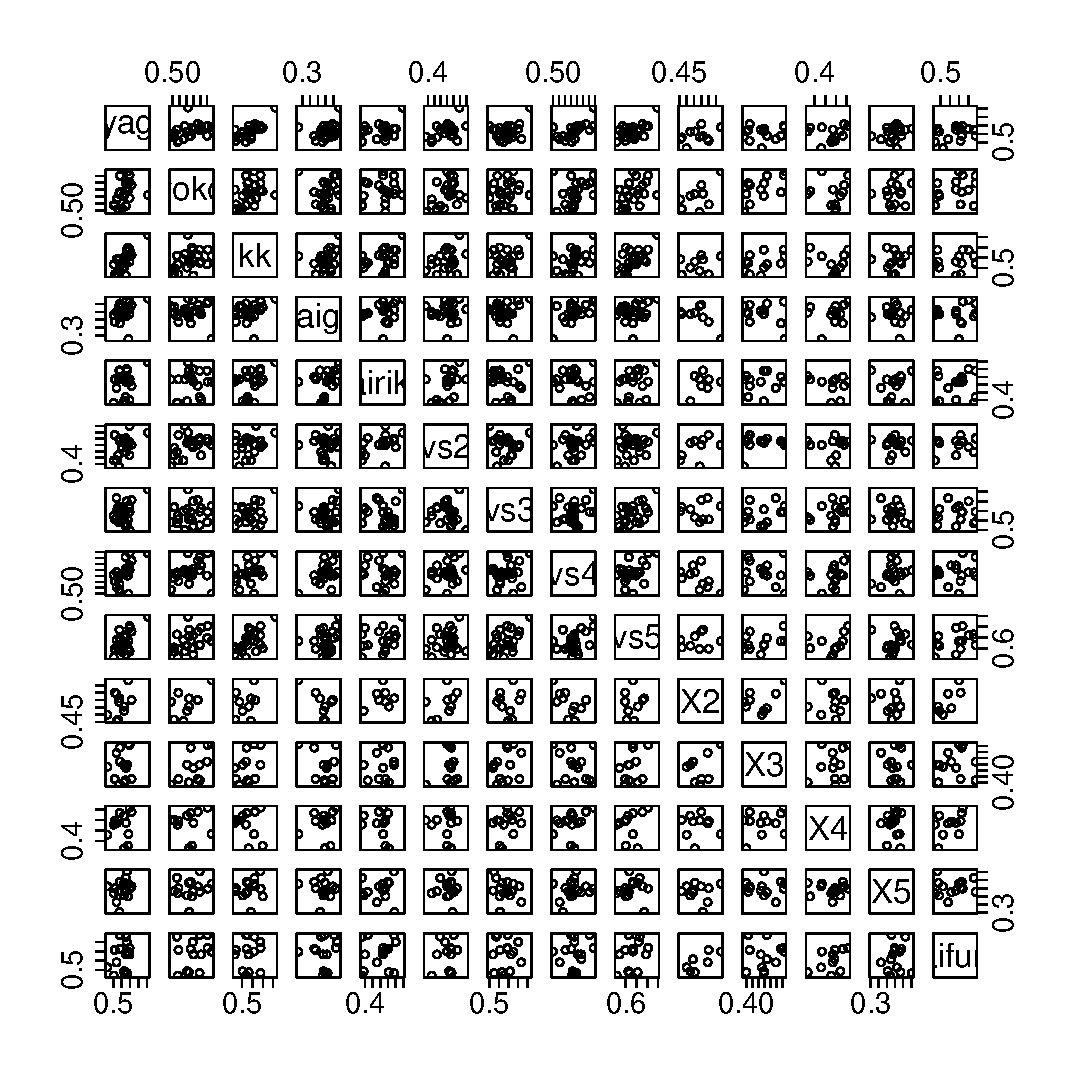
\includegraphics[width=1\textwidth]{graph/pairs-raw.eps}
\end{figure}
\\
 相関係数を調べると、居飛車系の戦法は居飛車系の戦法と正の相関が、振り飛車系の戦法とは負の相関があった。
振り飛車系戦法も同様に振り飛車との相関係数は正で、居飛車との相関係数は負となっていた。
\\

\section{主成分分析}
\subsection{分析結果}
データの空欄は指した回数の少ない戦法なので、一律に勝率は三割若しくは零割としてbiplotを描いた。
\\
 今回のデータは勝率でとっていて、戦型ごとの分散の違いは残しておきたい情報なので標準化は行っていない。
\\
\begin{figure}[h]
    \begin{tabular}{cc}
        \begin{minipage}[t]{0.47\hsize}
            \centering
            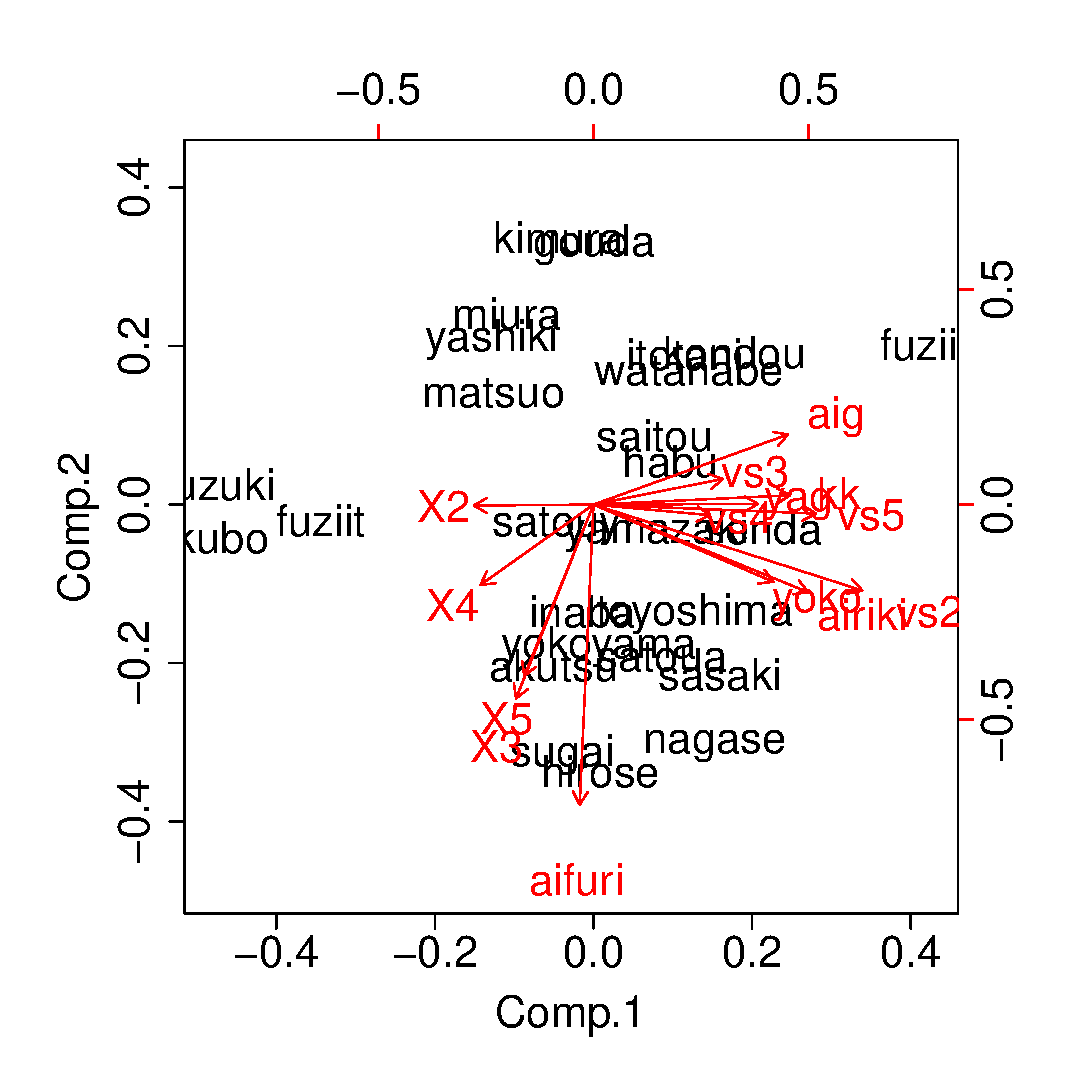
\includegraphics[width=0.9\textwidth]{graph/shougi-biplot.eps}
            \caption{苦手戦法の勝率三割}
        \end{minipage}
        \begin{minipage}[t]{0.47\hsize}
            \centering
            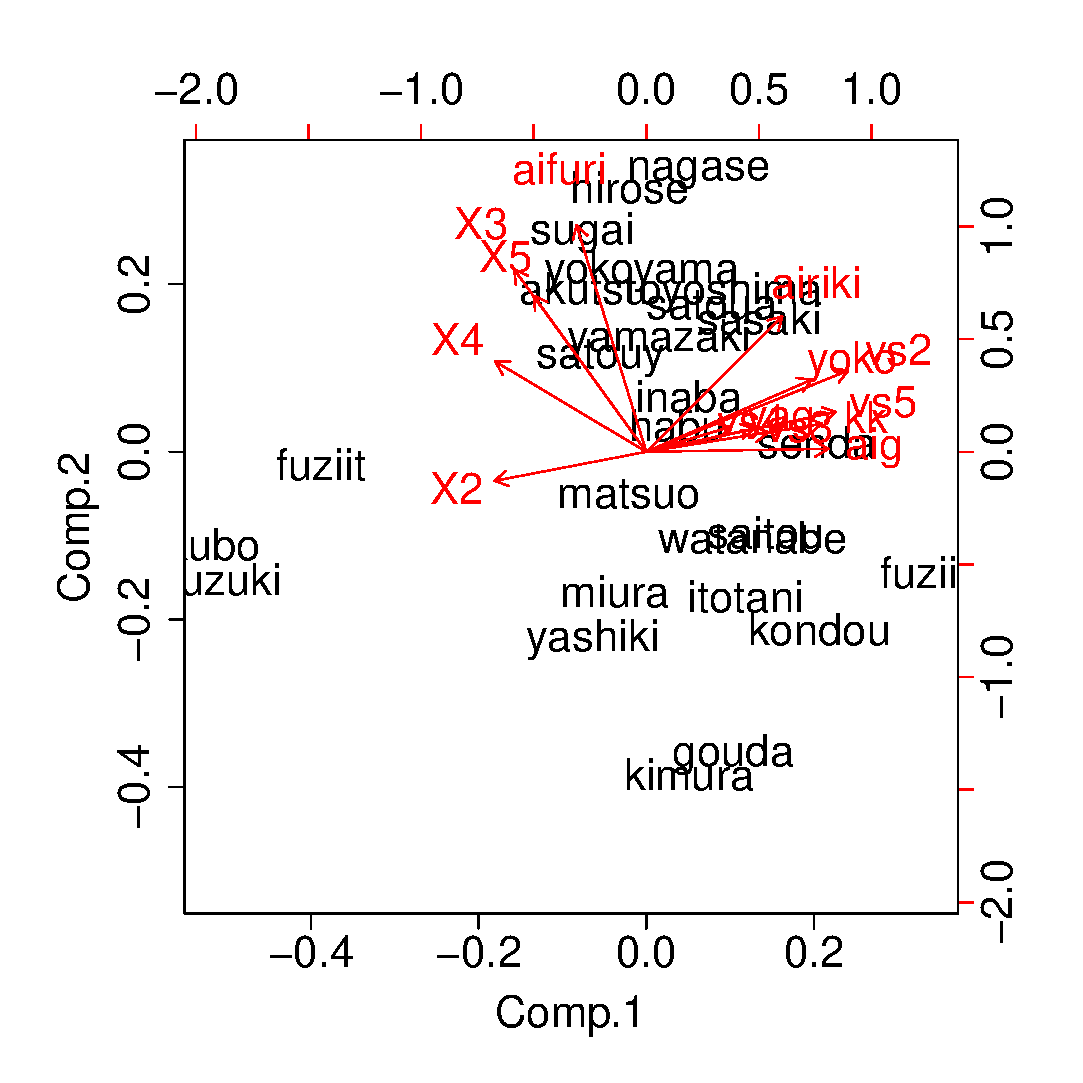
\includegraphics[width=0.9\textwidth]{graph/shougi-biplot0.eps}
            \caption{苦手戦法の勝率零割}
        \end{minipage}
    \end{tabular}
\end{figure}
\\
 第二主成分の向きが逆になるだけでどちらもほぼ変わりなかったので、勝率三割とした方をみることにする。
\\
 次に寄与率を見る。
\\
\begin{tabular}{l||c|c|c|c|c}
    & Comp.1 & Comp.2 & Comp.3 & Comp.4 & Comp.5 \\ \hline
Standard deviation & 0.3475536 & 0.2485964 & 0.1906889 & 0.15845832 & 0.14708448 \\
Proportion of Variance & 0.3777952 & 0.193287 & 0.1137271 & 0.07853134 & 0.06766228 \\
Cumulative Proportion  & 0.3777952 & 0.5710822 & 0.6848093 & 0.76334062 & 0.8310029 \\    
\end{tabular}
\\
\\
\\
\begin{tabular}{l||c|c|c|c|c}
    & Comp.6 & Comp.7 & Comp.8 & Comp.9 & Comp.10 \\ \hline
    Standard deviation & 0.12627479 & 0.10243472 & 0.08998564 & 0.08330242 & 0.06901344 \\
    Proportion of Variance & 0.04987079 & 0.03281764 & 0.02532558 & 0.02170342 & 0.01489636 \\
    Cumulative Proportion & 0.88087369 & 0.91369132 & 0.9390169 & 0.96072032 & 0.97561669 \\
\end{tabular}
\\
\\
\\
\begin{tabular}{l||c|c|c|c|}
    & Comp.11 & Comp.12 & Comp.13 & Comp.14 \\ \hline
    Standard deviation & 0.052578537 & 0.046174839 & 0.040563618 & 0.035413523 \\
    Proportion of Variance & 0.008646292 & 0.006668431 & 0.005146195 & 0.003922394 \\
    Cumulative Proportion & 0.984262979 & 0.990931411 & 0.996077606 & 1.000000000 \\   
\end{tabular}
\\
\\
主成分負荷は以下のようになる。

\begin{minipage}[t]{0.47\hsize}
    \centering
    \includegraphics[width=2.5\textwidth]{graph/loadings-shougi-pc.jpg}
\end{minipage}
\\\\\\\\\\\\\\\\\\\\\
 主成分得点も記す。
\\
\begin{tabular}{cc}
    \begin{minipage}[t]{0.47\hsize}
        \centering
        \includegraphics[width=1\textwidth]{graph/shogi-scores-1.jpg}
    \end{minipage}
    \begin{minipage}[t]{0.47\hsize}
        \centering
        \includegraphics[width=1\textwidth]{graph/shogi-scores-2.jpg}
    \end{minipage}
\end{tabular}
\begin{minipage}[t]{0.47\hsize}
    \includegraphics[width=1\textwidth]{graph/shogi-scores-3.jpg}
\end{minipage}
\subsection{解釈}
\begin{itemize}
    \item 右に行くほど勝率の高い棋士が並ぶので第一主成分は棋力とわかる。
    実際、第一主成分得点は藤井聡太二冠が飛び抜けて大きく(値は0.75なので図に収まっていない)、以下A級(リーグ戦のトップ)棋士やタイトルホルダーが並んでいる。
    \item 下側の棋士ほど振り飛車を指しこなす棋士なので第二主成分は振り飛車党か否かを表している。
    \item 第一主成分への寄与を見ると、相居飛車の戦型がもっとも重く(約0.3ずつ)、次に対抗系の居飛車側(0.19から0.44)、
    そして振り飛車系は負(-0.1から-0.2)で加算されていた。
    つまり居飛車が得意な棋士は振り飛車党の棋士より強い傾向にあるとわかる。
    \item 三間飛車(X3)と中飛車(X5)はほぼ同じ向きを向いているが、
    三間飛車と中飛車は攻撃的な振り飛車と言う点で似ていてそれが反映されている。
    また、相振り飛車は上の図3でも示したように、飛車が向かい合わないという点で相居飛車と似ているのもbiplotの図でみてとれる。
    \item 近年将棋AIがかなり強くなったが、将棋AIも飛車を序盤に降っただけで評価値をマイナスにするので、それと同じ結果が出ている。
    \item また主成分の寄与率はなかなか増えなかった。
    第二主成分までの累積寄与率も0.571までしか行かなかった。
    戦型を細かく分類して変数が増えすぎたのかと思い、
    棋士のデータを増やしたがそれでも累積寄与率はあまり変わらなかった。
    \item 第三主成分は相居飛車力戦と中飛車、四間飛車が正に、相振り飛車が負に加算されていた。
    また第三主成分得点を調べても羽生九段と菅井八段が約0.3と大きく、
    稲葉八段、佐藤天彦九段、齋藤八段が-0.4から-0.3と小さくなって、戦型の観点でも棋士の観点でも
    第三主成分の解釈はできなかった。

\end{itemize}

\end{document}